\subsection{Finding \texorpdfstring{$T_{2}^*$}{T2*} for Water, Ethanol and Rubber} \label{B2}

Similar to Section \ref{B1}, the FID of three samples (doped water, ethanol, and rubber) were measured for 90 degree pulses only. The repetition rate, detector phase, and pulse value were set to maximize the signal for each sample.\\

The magnetization as a function of time for the FID experiment is given by the expression,
\begin{align*}
    M_y(t) &= M_0 e^{-t/T_2^*} \numberthis\label{eqn:B2:eqn1} \\
    \intertext{Taking the natural logarithm of both sides of this expression,}
    \ln(M_y(t)) &= -t/T_2^* + \ln(M_0) \numberthis \label{eqn:B2:logfit}
\end{align*}

The first method to calculate $T_2^*$ is an approximation method. From Equation \ref{eqn:B2:eqn1}, when $t=T_2^*$ the magnetization is $M_y=M_0/e$; thus by calculating the time where the magnetization has decayed to this value is an approximate value of $T_2^*$. From the FID of each sample, the peak magnetization $M_0$ is measured and the intersection of the decay slope with $M_0/e$ is calculated. This is demonstrated in Figure \ref{fig:B2:T2*_approx} for doped water, and the estimated values of $T_2^*$ are summarized in Table \ref{tab:B2:T2*_values} (see Figure \ref{fig:A_B2_estimate} in Appendix for $T_2^*$ estimation plots for ethanol and rubber). The uncertainty values in our estimated time constant are taken as the uncertainty in determining $M_0$. This method is highly inaccurate, and is used only as an initial estimation.
\begin{figure}[H]
\centering
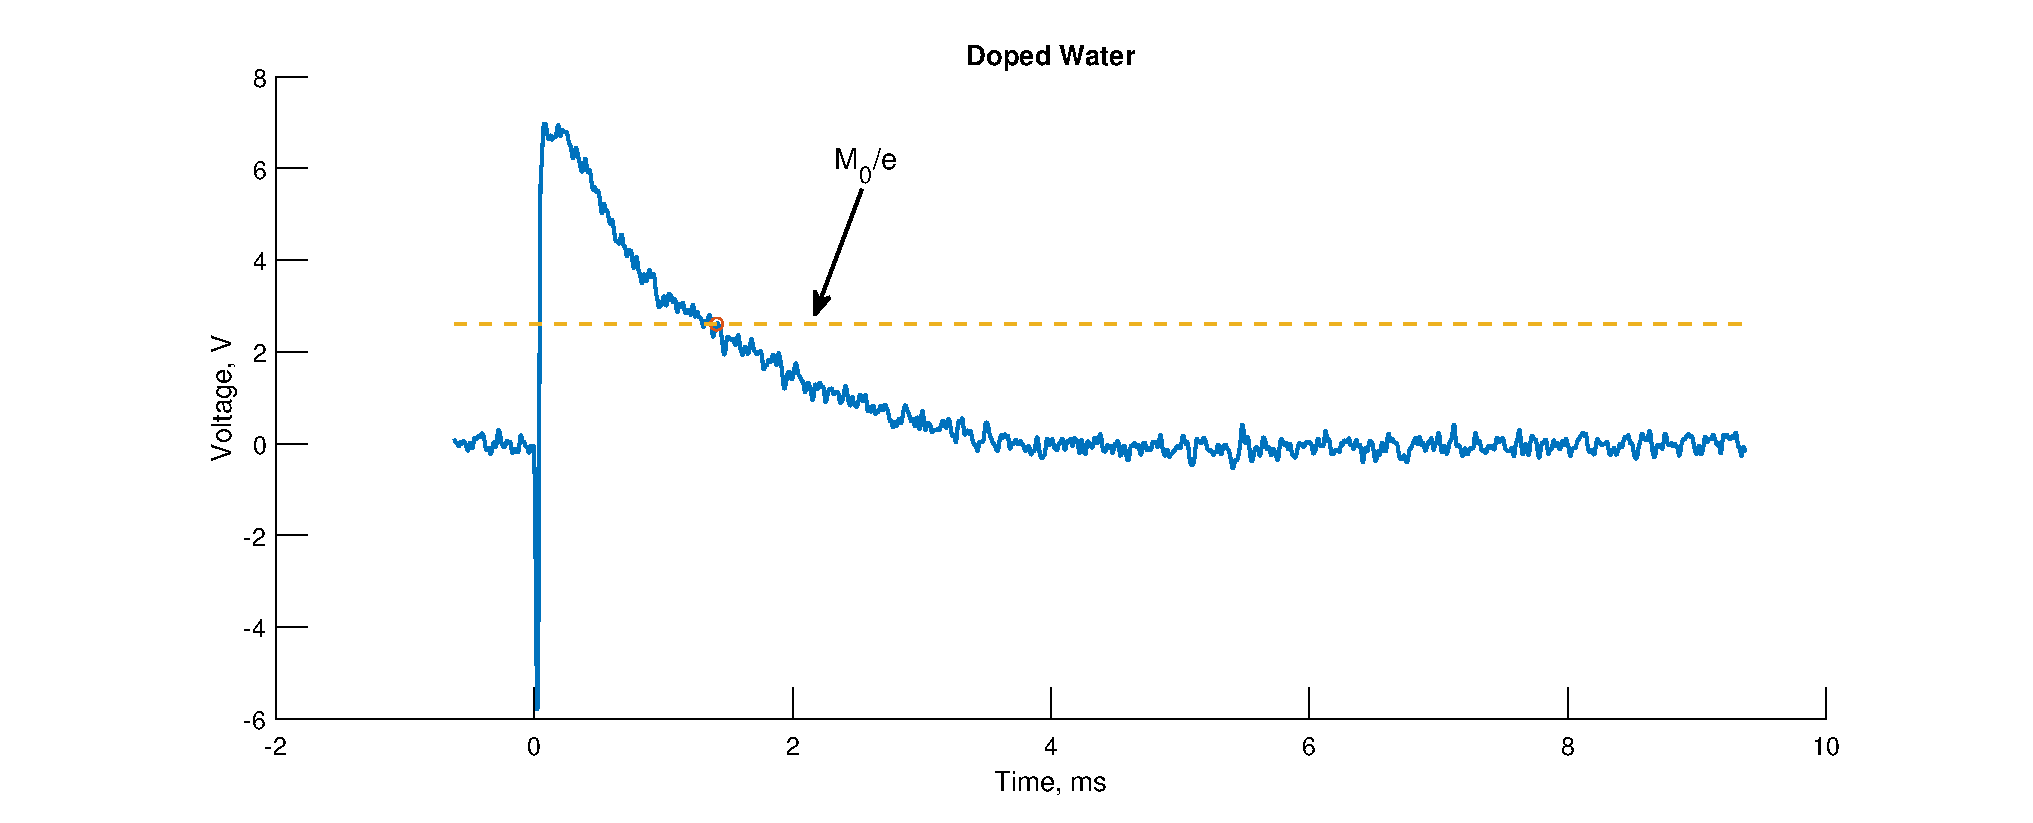
\includegraphics[width=\textwidth]{figures/B2/B2_2.eps}
\caption{Estimation of $T_2^*$ for doped water using the time value where $M_y\approx M_0/e$. Values for other samples are tabulated in Table \ref{tab:B2:T2*_values}.}
\label{fig:B2:T2*_approx}
\end{figure}

A more accurate method of calculating the time constant $T_2^*$ is to use a linear fit with the form of Equation \ref{eqn:B2:logfit}. Prior to fitting, each data set was zero shifted; and no filtering was performed for these data sets. The natural logarithm of the magnetization was fit with a linear slope using the method of least squares. Only the portion of the data set which contained a strong signal was used in the fitting process, as the signal to noise ratio with the rest of the data set is too low to generate an accurate value of $T_2^*$. The uncertainty in these measurements are regarded as the 95\% confidence interval of the fitting algorithm. Figure \ref{fig:B2:T2*_samples} demonstrates the fits for each sample (note that this plot demonstrates the fit data converted back to exponential form, to demonstrate the accuracy of the fit to the raw data).\\

\begin{figure}[H]
\centering
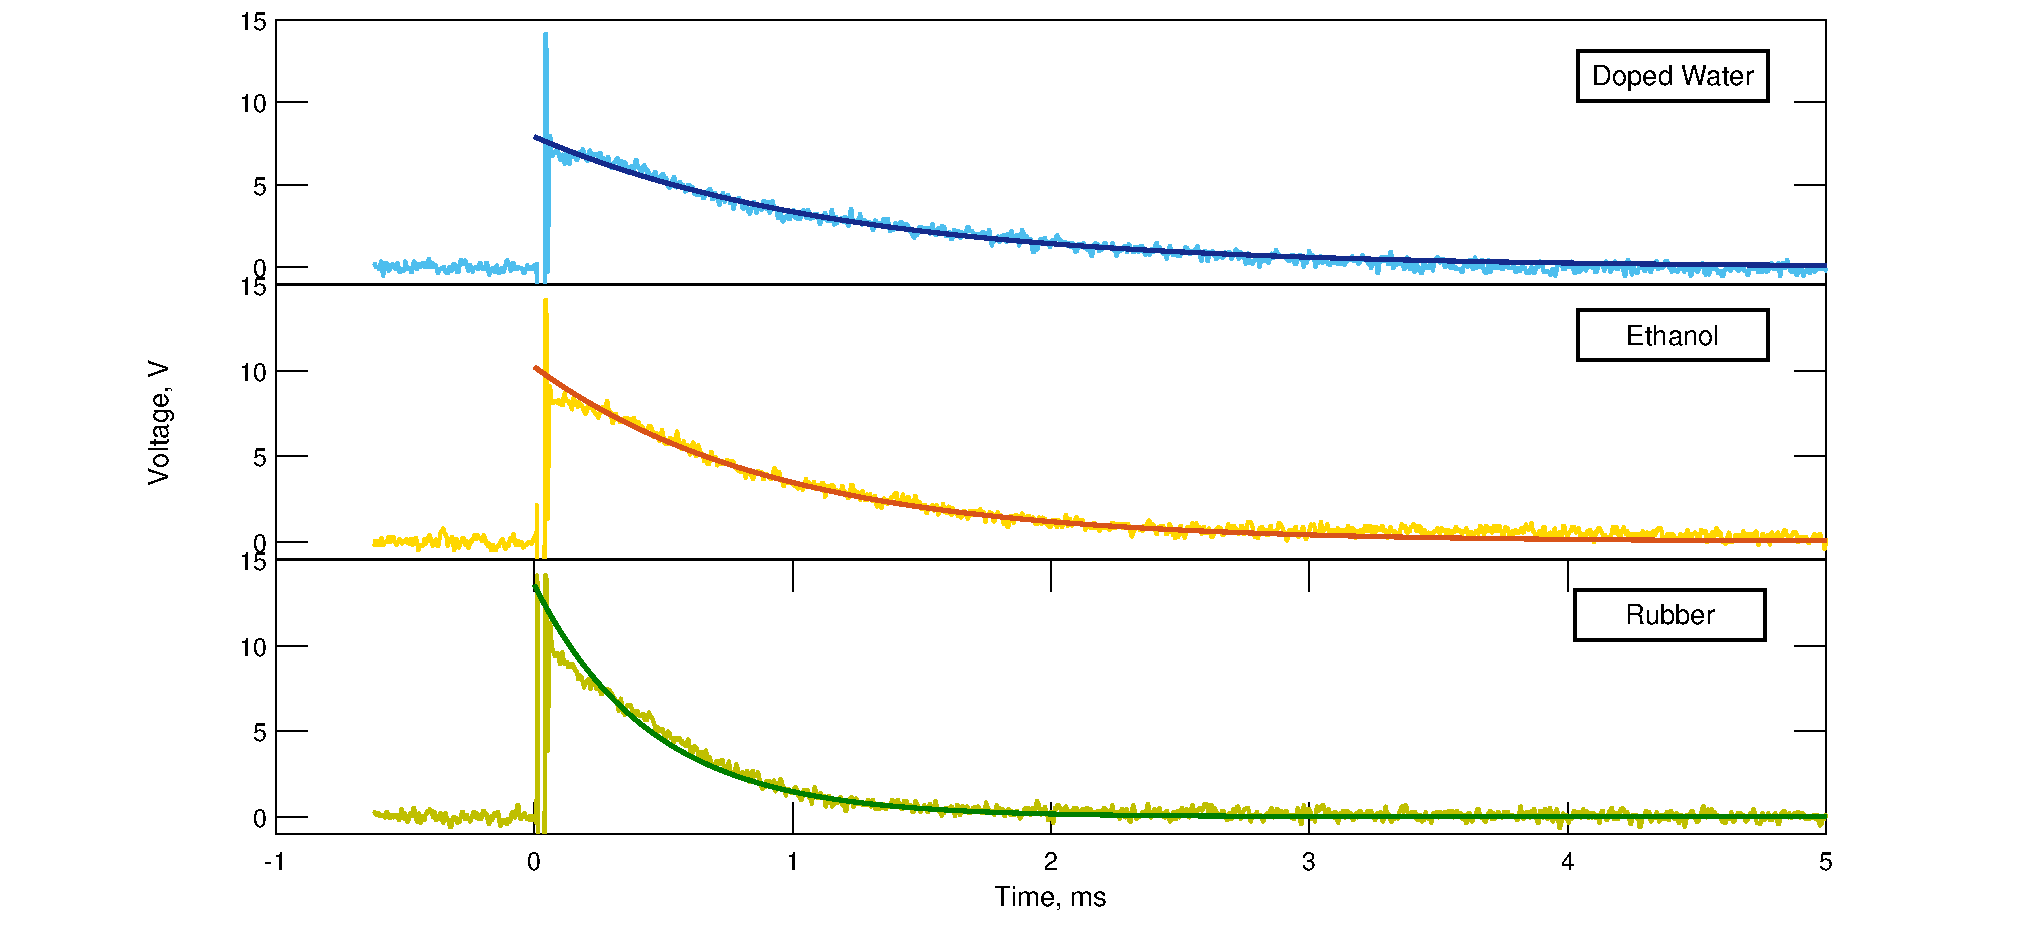
\includegraphics[width=\textwidth]{figures/B2/B2_1.eps}
\caption{FID from a 90 degree pulse for doped water, ethanol, and rubber to determine $T_2^*$.}
\label{fig:B2:T2*_samples}
\end{figure}

The behaviour of each fit matches quite well with the experimental data, following the trend very closely. The $R^2$ values in Table \ref{tab:B2:T2*_values} are based off of the linear fit to the natural logarithm (see Figure \ref{fig:A_B2_logfit} in the Appendix).\\

For each sample, directly following the pulse there is a reduction in the peak value from what the theoretical model predicts. This is likely caused by cross-talk effects between the applied pulse and detector -- which is a systematic instrument error and could be reduced by readjusting the spectrometer settings. It could also be that there may be a better method to remove the detector peak.

\begin{table}[H]
    \centering
    \begin{tabular}{c|c|c|c|c}
    \toprule
    \textbf{Sample} & $T_2^*$ Estimate & $T_2^*$ (ms) & $R^2$ & Percent Difference (\%) \\ \midrule
        Doped Water & $1.4110\pm0.1472$ & $1.169 \pm 0.017$ & $0.9324$  & $18.76$\\
        Ethanol & $1.2270\pm0.1472$ & $0.9239 \pm 0.0085$ & $0.9638$ & $28.18$\\
        Rubber & $0.6415\pm0.1104$ & $0.4495 \pm 0.0073$ & $0.9550$  & $35.20$ \\ \bottomrule
    \end{tabular}
    \caption{Summarized values of $T_2^*$ for the three samples. First column is calculated using th estimation of $M_y=M_0/e$, depicted in Figure \ref{fig:B2:T2*_approx}. The second column is calculated from the fits depicted in Figure \ref{fig:B2:T2*_samples}, with the corresponding $R^2$ goodness-of-fit value.}
    \label{tab:B2:T2*_values}
\end{table}

Comparing the two methods summarized in Table \ref{tab:B2:T2*_values}, we see that the estimated value of $T_2^*$ is always greater than the calculation using a fit. 


%Its possible that this is caused by deconstructive interference from the sharp peak that we see from the instrument? I remember it creates a peak like a damped harmonic oscillator and may have some effect like we see. I'll have to actually look at the scans we took before establishing this for sure.